\documentclass[14pt]{extbook}
\usepackage{multicol, enumerate, enumitem, hyperref, color, soul, setspace, parskip, fancyhdr} %General Packages
\usepackage{amssymb, amsthm, amsmath, latexsym, units, mathtools} %Math Packages
\everymath{\displaystyle} %All math in Display Style
% Packages with additional options
\usepackage[headsep=0.5cm,headheight=12pt, left=1 in,right= 1 in,top= 1 in,bottom= 1 in]{geometry}
\usepackage[usenames,dvipsnames]{xcolor}
\usepackage{dashrule}  % Package to use the command below to create lines between items
\newcommand{\litem}[1]{\item#1\hspace*{-1cm}\rule{\textwidth}{0.4pt}}
\pagestyle{fancy}
\lhead{Progress Quiz 10}
\chead{}
\rhead{Version C}
\lfoot{5170-5105}
\cfoot{}
\rfoot{Summer C 2021}
\begin{document}

\begin{enumerate}
\litem{
Determine the vertical asymptotes and holes in the rational function below.\[ f(x) = \frac{12x^{3} +25 x^{2} -48 x -45}{12x^{2} +17 x + 6} \]\begin{enumerate}[label=\Alph*.]
\item \( \text{Vertical Asymptote of } x = -0.667 \text{ and hole at } x = -0.75 \)
\item \( \text{Vertical Asymptotes of } x = -0.667 \text{ and } x = 1.667 \text{ with a hole at } x = -0.75 \)
\item \( \text{Vertical Asymptotes of } x = -0.667 \text{ and } x = -0.75 \text{ with no holes.} \)
\item \( \text{Vertical Asymptote of } x = 1.0 \text{ and hole at } x = -0.75 \)
\item \( \text{Holes at } x = -0.667 \text{ and } x = -0.75 \text{ with no vertical asymptotes.} \)

\end{enumerate} }
\litem{
Determine the vertical asymptotes and holes in the rational function below.\[ f(x) = \frac{4x^{3} -16 x^{2} -25 x + 100}{6x^{2} +11 x -10} \]\begin{enumerate}[label=\Alph*.]
\item \( \text{Holes at } x = 0.667 \text{ and } x = -2.5 \text{ with no vertical asymptotes.} \)
\item \( \text{Vertical Asymptote of } x = 0.667 \text{ and hole at } x = -2.5 \)
\item \( \text{Vertical Asymptotes of } x = 0.667 \text{ and } x = -2.5 \text{ with no holes.} \)
\item \( \text{Vertical Asymptote of } x = 0.667 \text{ and hole at } x = -2.5 \)
\item \( \text{Vertical Asymptotes of } x = 0.667 \text{ and } x = 2.5 \text{ with a hole at } x = -2.5 \)

\end{enumerate} }
\litem{
Which of the following functions \textit{could} be the graph below?
\begin{center}
    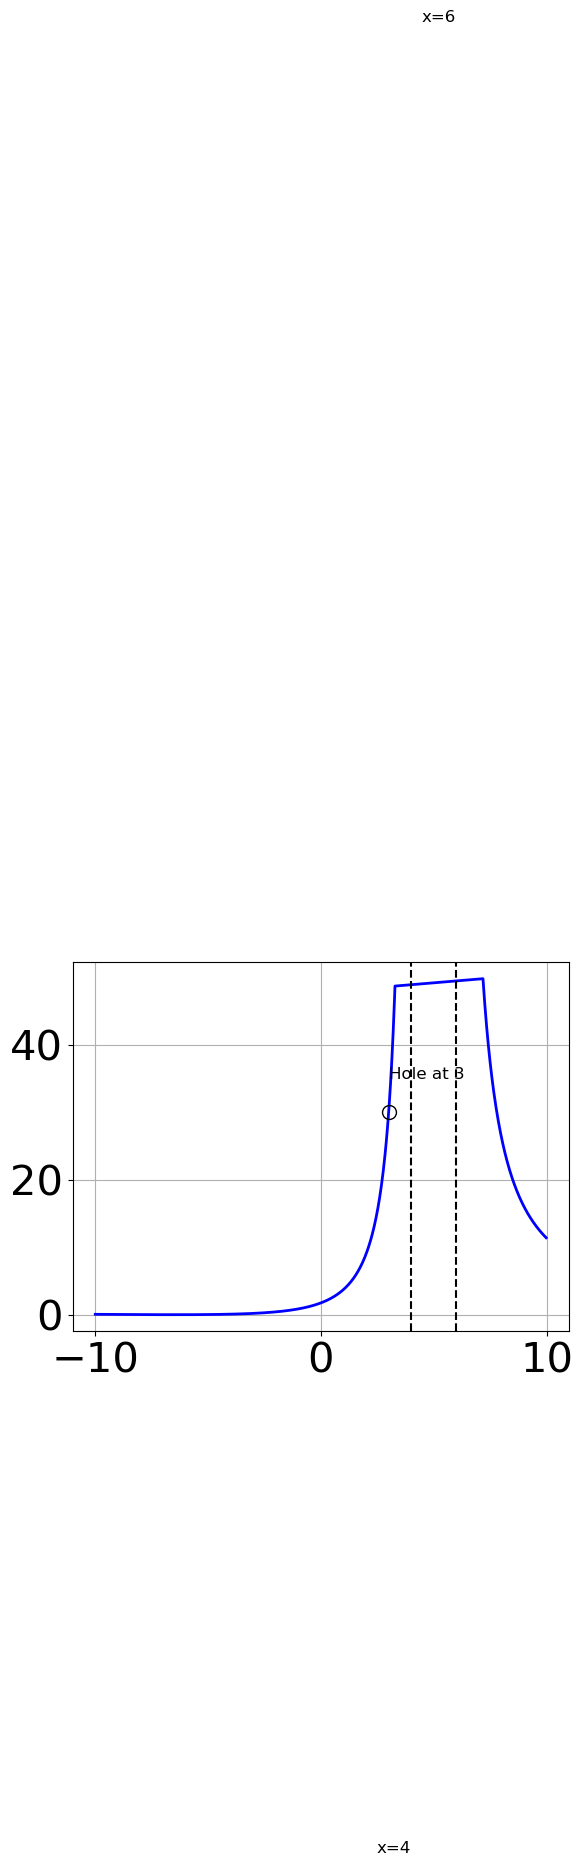
\includegraphics[width=0.5\textwidth]{../Figures/identifyGraphOfRationalFunctionCopyC.png}
\end{center}
\begin{enumerate}[label=\Alph*.]
\item \( f(x)=\frac{x^{3} -10.0 x^{2} +3.0 x + 126.0}{x^{3} +13.0 x^{2} +54.0 x + 72.0} \)
\item \( f(x)=\frac{x^{3} +10.0 x^{2} +3.0 x -126.0}{x^{3} -13.0 x^{2} +54.0 x -72.0} \)
\item \( f(x)=\frac{x^{3} +12.0 x^{2} +29.0 x -42.0}{x^{3} -13.0 x^{2} +54.0 x -72.0} \)
\item \( f(x)=\frac{x^{3} -11.0 x^{2} +16.0 x + 84.0}{x^{3} +13.0 x^{2} +54.0 x + 72.0} \)
\item \( \text{None of the above are possible equations for the graph.} \)

\end{enumerate} }
\litem{
Determine the vertical asymptotes and holes in the rational function below.\[ f(x) = \frac{12x^{3} +41 x^{2} +40 x + 12}{16x^{2} -9} \]\begin{enumerate}[label=\Alph*.]
\item \( \text{Vertical Asymptote of } x = 0.75 \text{ and hole at } x = -0.75 \)
\item \( \text{Vertical Asymptote of } x = 0.75 \text{ and hole at } x = -0.75 \)
\item \( \text{Vertical Asymptotes of } x = 0.75 \text{ and } x = -0.75 \text{ with no holes.} \)
\item \( \text{Vertical Asymptotes of } x = 0.75 \text{ and } x = -0.667 \text{ with a hole at } x = -0.75 \)
\item \( \text{Holes at } x = 0.75 \text{ and } x = -0.75 \text{ with no vertical asymptotes.} \)

\end{enumerate} }
\litem{
Determine the horizontal and/or oblique asymptotes in the rational function below.\[ f(x) = \frac{12x^{3} -37 x^{2} -3 x + 18}{4x^{2} +5 x -6} \]\begin{enumerate}[label=\Alph*.]
\item \( \text{Horizontal Asymptote of } y = -2.0 \text{ and Oblique Asymptote of } y = 3x -13 \)
\item \( \text{Horizontal Asymptote of } y = 3.0 \text{ and Oblique Asymptote of } y = 3x -13 \)
\item \( \text{Horizontal Asymptote at } y = -2.0 \)
\item \( \text{Oblique Asymptote of } y = 3x -13. \)
\item \( \text{Horizontal Asymptote of } y = 3.0  \)

\end{enumerate} }
\litem{
Determine the horizontal and/or oblique asymptotes in the rational function below.\[ f(x) = \frac{4x^{3} -4 x^{2} -23 x + 30}{-6x^{3} +8 x^{2} +17 x -30} \]\begin{enumerate}[label=\Alph*.]
\item \( \text{Horizontal Asymptote of } y = -0.667  \)
\item \( \text{Vertical Asymptote of } y = 2  \)
\item \( \text{Vertical Asymptote of } y = -1.667  \)
\item \( \text{Horizontal Asymptote of } y = 0  \)
\item \( \text{None of the above} \)

\end{enumerate} }
\litem{
Determine the vertical asymptotes and holes in the rational function below.\[ f(x) = \frac{6x^{3} -37 x^{2} +75 x -50}{12x^{2} -35 x + 25} \]\begin{enumerate}[label=\Alph*.]
\item \( \text{Vertical Asymptotes of } x = 1.25 \text{ and } x = 1.667 \text{ with no holes.} \)
\item \( \text{Vertical Asymptote of } x = 0.5 \text{ and hole at } x = 1.667 \)
\item \( \text{Vertical Asymptotes of } x = 1.25 \text{ and } x = 2.5 \text{ with a hole at } x = 1.667 \)
\item \( \text{Holes at } x = 1.25 \text{ and } x = 1.667 \text{ with no vertical asymptotes.} \)
\item \( \text{Vertical Asymptote of } x = 1.25 \text{ and hole at } x = 1.667 \)

\end{enumerate} }
\litem{
Determine the horizontal and/or oblique asymptotes in the rational function below.\[ f(x) = \frac{12x^{3} +59 x^{2} +79 x + 30}{4x^{2} -7 x -15} \]\begin{enumerate}[label=\Alph*.]
\item \( \text{Horizontal Asymptote at } y = 3.0 \)
\item \( \text{Oblique Asymptote of } y = 3x + 20. \)
\item \( \text{Horizontal Asymptote of } y = 3.0  \)
\item \( \text{Horizontal Asymptote of } y = 3.0 \text{ and Oblique Asymptote of } y = 3x + 20 \)
\item \( \text{Horizontal Asymptote of } y = 3.0 \text{ and Oblique Asymptote of } y = 3x + 20 \)

\end{enumerate} }
\litem{
Determine the horizontal and/or oblique asymptotes in the rational function below.\[ f(x) = \frac{30x^{3} -163 x^{2} +187 x -60}{-20x^{3} +34 x^{2} -94 x + 24} \]\begin{enumerate}[label=\Alph*.]
\item \( \text{Horizontal Asymptote of } y = 0  \)
\item \( \text{Horizontal Asymptote of } y = -1.500  \)
\item \( \text{Vertical Asymptote of } y = 4  \)
\item \( \text{None of the above} \)
\item \( \text{Vertical Asymptote of } y = 0.500  \)

\end{enumerate} }
\litem{
Which of the following functions \textit{could} be the graph below?
\begin{center}
    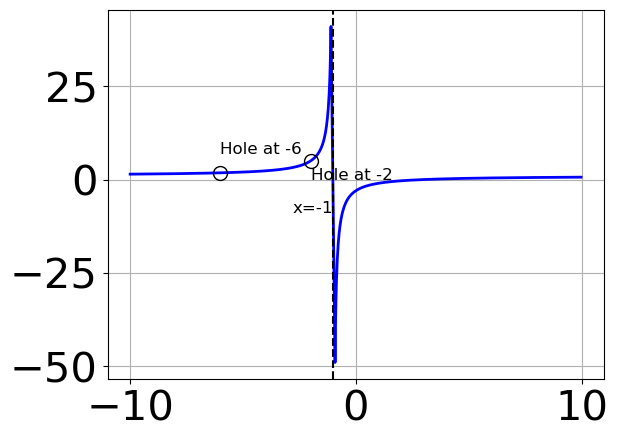
\includegraphics[width=0.5\textwidth]{../Figures/identifyGraphOfRationalFunctionC.png}
\end{center}
\begin{enumerate}[label=\Alph*.]
\item \( f(x)=\frac{x^{3} +5.0 x^{2} -12.0 x -36.0}{x^{3} +9.0 x^{2} +20.0 x + 12.0} \)
\item \( f(x)=\frac{x^{3} -5.0 x^{2} -12.0 x + 36.0}{x^{3} -9.0 x^{2} +20.0 x -12.0} \)
\item \( f(x)=\frac{x^{3} +6.0 x^{2} +11.0 x + 6.0}{x^{3} -9.0 x^{2} +20.0 x -12.0} \)
\item \( f(x)=\frac{x^{3} +6.0 x^{2} -7.0 x -60.0}{x^{3} +9.0 x^{2} +20.0 x + 12.0} \)
\item \( \text{None of the above are possible equations for the graph.} \)

\end{enumerate} }
\end{enumerate}

\end{document}